\ylDisplay{Elektriskeem} % Ülesande nimi
{Kristian Kuppart} % Autor
{lahtine} % Voor
{2016} % Aasta
{G 3} % Ülesande nr.
{3} % Raskustase
{
% Teema: Elektriahelad
\ifStatement

Leidke juuresoleval skeemil voolutugevus $I$ läbi ampermeetri kahel juhul: vahetult pärast lüliti sulgemist ja pika aja möödumisel. Eeldada, et kondensaatorid on enne lüliti sulgemist laadimata. Patarei lugeda ideaalseks.
\begin{center}
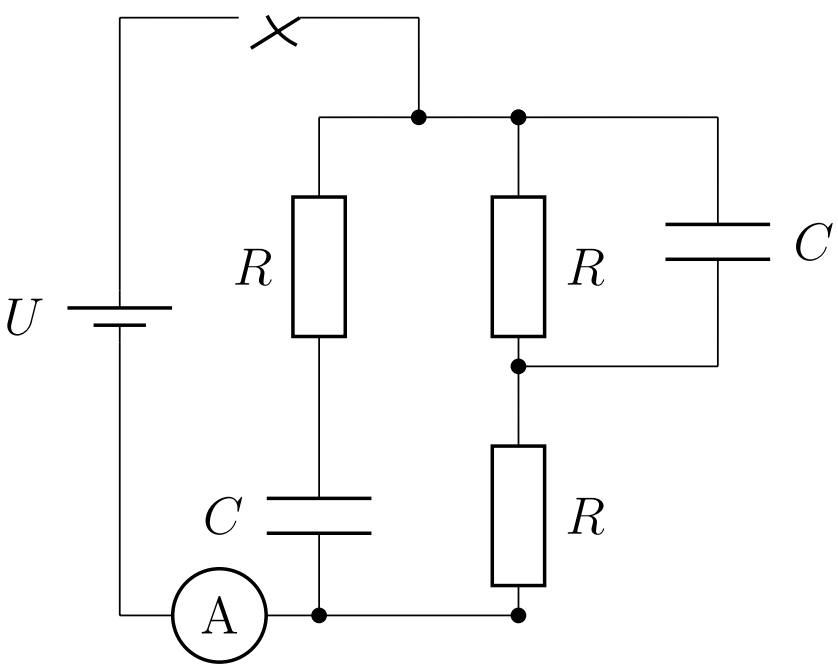
\includegraphics[width=0.45\textwidth]{2016-lahg-03-skeemjoonis.png}
\end{center}
\fi


\ifHint
Kuna kondensaatorid on enne lüliti sulgemist laadimata, on ka pinge nende klemmidel $0$.\\
Pärast pika aja möödumist on kondensaatorite laeng jõudnud stabiliseerida ehk vool läbi kondensaatorite on $0$. Teisisõnu võib kondensaatorid efektiivselt skeemist lahti ühendada.
\fi


\ifSolution
Vahetult pärast lüliti sulgemist ei ole parempoolsele kondensaatorile laengut jõudnud koguneda, mis tähendab, et pinge tema klemmidel $U=\frac{q}{C}=0$. Parempoolsest ülemisest takistist esimesel hetkel voolu läbi ei lähe. Sama  mõttekäik kehtib vasakpoolse kondensaator kohta, niisiis voolutugevus $I=\frac{2U}{R}$ 

Pika aja möödumisel on mõlemad kondensaatorid efektiivselt lahti ühendatud, kogu vool läheb läbi keskmise haru: $I=\frac{U}{2R}$
\fi


\ifEngStatement
% Problem name: Circuit diagram
Find the current strength $I$ in the given drawing through the ammeter for two cases: directly after closing the switch and after a long time has passed since closing the switch. Assume that the capacitors are uncharged before closing the switch. The battery is ideal. 
\begin{center}
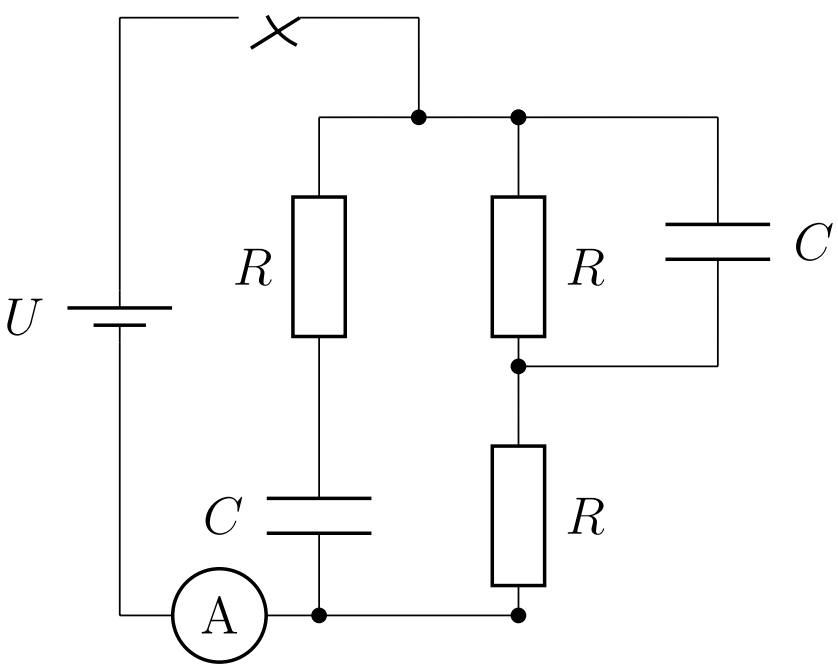
\includegraphics[width=0.45\textwidth]{2016-lahg-03-skeemjoonis}
\end{center}
\fi


\ifEngHint
Because the capacitors are uncharged before closing the switch the voltage on their terminals is $0$.\\
After a long time has passed the charge of the capacitors has managed to even out meaning that the current through the capacitors is $0$. In other words the capacitors can be effectively cut out from the diagram.
\fi


\ifEngSolution
Momentarily after closing the switch charge has not yet managed to accumulate on the right capacitor meaning that the voltage on its leads is $U=\frac{q}{C}=0$. In the first moment no current goes through the upper right resistor. The same reasoning applies to the left capacitor, so the current is $I=\frac{2U}{R}$.\\
After a long time has passed both of the capacitors have been effectively disconnected and the total current goes through the middle branch: $I=\frac{U}{2R}$.
\fi
}